\documentclass[11pt]{article}
\usepackage[margin=0.9in]{geometry}
\usepackage{amsmath, amssymb}
\usepackage{graphicx}
\usepackage{booktabs}
\usepackage{caption}
\usepackage[hidelinks]{hyperref}
\usepackage{enumitem}
\setlist{nosep, leftmargin=1.4em}
\setlength{\parskip}{4pt}
\setlength{\parindent}{0pt}
\captionsetup{font=small}

\title{\vspace{-2em}Naive Bayes and SVD}
\author{Derek}
\date{}

\begin{document}
\maketitle
\vspace{-3em}

All code is in \texttt{hw\_bayes\_svd.py} (NumPy + Matplotlib only; the classifier is written from scratch).

\section{Gaussian Naive Bayes on MNIST}

\textbf{Steps in the code.}
\begin{enumerate}
  \item \textbf{Load} the four MNIST IDX files (60{,}000 train, 10{,}000 test), flatten each $28\times28$ image to $\mathbf{x}\in\mathbb{R}^{784}$, and scale pixels to $[0,1]$.
  \item \textbf{Fit}: for each digit $c$, estimate the prior $\hat\pi_c = N_c/N$ and, for every pixel $d$, a mean $\mu_{c,d}$ and variance $\sigma^2_{c,d}$.
  \item \textbf{Smooth}: add $\varepsilon = \alpha\cdot\max_d \operatorname{Var}(x_d)$ to every variance. Around 200 border pixels per class are always 0, so their variance is exactly 0 and the Gaussian would give likelihood 0 to any test image with a stray pixel there.
  \item \textbf{Predict} the class with the largest log-posterior (logs avoid underflow from multiplying 784 densities):
  \[
    \hat y = \arg\max_c \Big[\log\hat\pi_c - \tfrac12\sum_{d=1}^{784}\log(2\pi\sigma^2_{c,d}) - \tfrac12\sum_{d=1}^{784}\frac{(x_d-\mu_{c,d})^2}{\sigma^2_{c,d}}\Big].
  \]
  \item \textbf{Tune} $\alpha$ on a 10{,}000-image validation split taken from the training set, refit on all training data, then test once.
\end{enumerate}
Fit is $O(ND)$ time, prediction is $O(MCD)$, and the model stores $O(CD)$ numbers.

\textbf{Results.} With the usual default $\alpha=10^{-9}$ the test accuracy is 55.6\% (identical to scikit-learn's \texttt{GaussianNB}, which I used only as a check). Validation picked $\alpha=0.05$, which gives \textbf{81.4\% test accuracy}. The worst confusion is 4 predicted as 9 (Fig.~\ref{fig:conf}), which makes sense since their average shapes almost overlap.

\begin{figure}[h]
  \centering
  \begin{minipage}{0.42\textwidth}
    \centering
    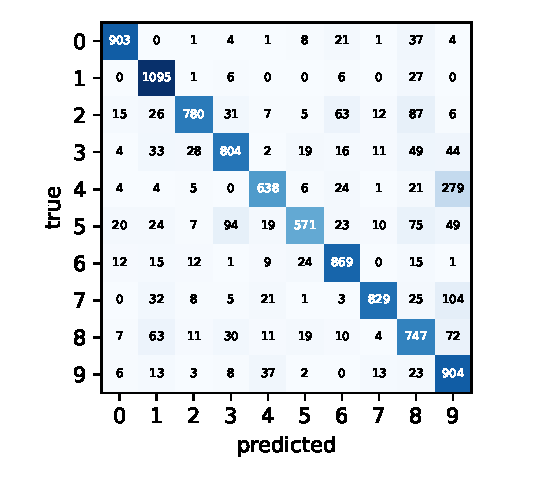
\includegraphics[width=\linewidth]{fig_confusion.pdf}
    \captionof{figure}{Test confusion matrix, $\alpha=0.05$.}
    \label{fig:conf}
  \end{minipage}\hfill
  \begin{minipage}{0.52\textwidth}
    \centering
    \small
    \begin{tabular}{lc}
      \toprule
      Variance smoothing $\alpha$ & Validation acc. \\
      \midrule
      $10^{-9}$ & 56.5\% \\
      $10^{-4}$ & 67.5\% \\
      $10^{-2}$ & 77.5\% \\
      $0.05$    & \textbf{79.7\%} \\
      $0.1$     & 79.6\% \\
      $0.5$     & 75.8\% \\
      \bottomrule
    \end{tabular}
    \captionof{table}{Choosing $\alpha$ on held-out training data.}
  \end{minipage}
\end{figure}

\section{The idea behind Naive Bayes}

Bayes' rule turns the classification question ``which class is most likely given this image?'' into things we can estimate:
\[
  P(c\mid\mathbf{x}) = \frac{P(\mathbf{x}\mid c)\,P(c)}{P(\mathbf{x})} \;\propto\; P(\mathbf{x}\mid c)\,P(c).
\]
$P(\mathbf{x})$ is the same for every class, so it drops out of the argmax. The hard part is $P(\mathbf{x}\mid c)$, a joint distribution over 784 pixels: a full Gaussian would need a $784\times784$ covariance per class, which is too many parameters and is singular here anyway.

The \textbf{naive assumption} is that pixels are \emph{conditionally independent given the class}:
\[
  P(\mathbf{x}\mid c) = \prod_{d=1}^{784} P(x_d\mid c).
\]
This replaces one 784-dimensional problem with 784 one-dimensional ones.

\textbf{In my model:}
\begin{itemize}
  \item \textbf{Assumption:} each class keeps only a mean and a variance per pixel, i.e.\ a diagonal covariance with all pixel--pixel covariances set to 0. The product over pixels becomes the sum over pixels in the log-likelihood.
  \item \textbf{Prior:} $P(c)=N_c/N$, the class frequency in the training set (about $0.09$--$0.11$ each).
  \item \textbf{Likelihood:} $P(\mathbf{x}\mid c)=\prod_d \mathcal{N}(x_d;\,\mu_{c,d},\,\sigma^2_{c,d}+\varepsilon)$.
\end{itemize}

The assumption is clearly false for images. Within class 7, the centre pixel has correlation $0.82$ with the pixel below it, so a thick stroke counts as many independent pieces of evidence. This makes the model overconfident: 93\% of test predictions have posterior above $0.999$, yet only 84\% of those are right. Pixels also are not Gaussian (that pixel is exactly 0 in 72\% of 7s). These two errors explain why accuracy stalls around 80\%.

\section{SVD on CIFAR-10}

I stacked the 10{,}000 CIFAR-10 test images as rows of $A\in\mathbb{R}^{10000\times3072}$ ($32\cdot32\cdot3$ values each), subtracted the mean image, and computed the economy SVD $A=U\Sigma V^\top$ ($O(ND^2)$ time). The rank-$k$ reconstruction is
\[
  \hat A_k = \bar{\mathbf{a}} + U_k\Sigma_kV_k^\top,
\]
so each image is described by $k$ coefficients instead of 3072 pixels.

\begin{table}[h]
  \centering
  \small
  \begin{tabular}{ccccc}
    \toprule
    $k$ & Variance kept $\sum_{i\le k}\sigma_i^2/\sum_i\sigma_i^2$ & MSE & PSNR (dB) & Relative error \\
    \midrule
    10  & 65.7\% & 0.0209 & 16.8 & 0.586 \\
    50  & 84.8\% & 0.0092 & 20.4 & 0.390 \\
    75  & 88.4\% & 0.0070 & 21.5 & 0.341 \\
    100 & 90.7\% & 0.0056 & 22.5 & 0.305 \\
    500 & 98.9\% & 0.0007 & 31.8 & 0.104 \\
    \bottomrule
  \end{tabular}
  \caption{Reconstruction quality vs.\ $k$. The relative error equals $\sqrt{\sum_{i>k}\sigma_i^2}/\lVert A\rVert_F$ (Eckart--Young).}
\end{table}

\begin{figure}[h]
  \centering
  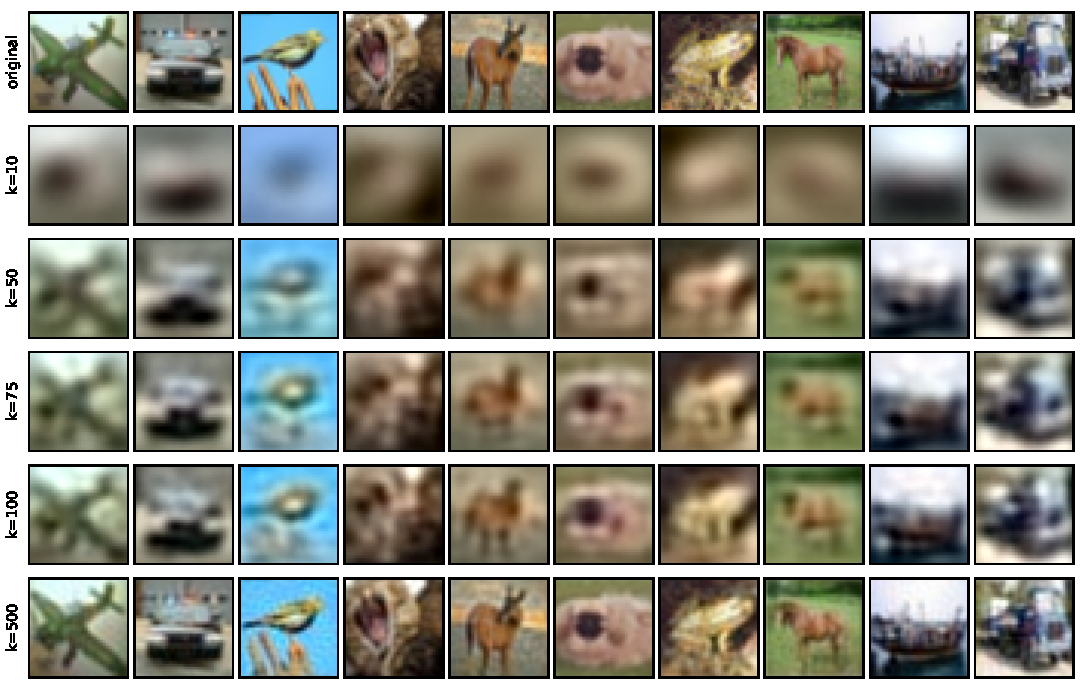
\includegraphics[width=0.72\textwidth]{fig_svd.pdf}
  \caption{One test image per class (top row) and its rank-$k$ reconstructions.}
  \label{fig:svd}
\end{figure}

At $k=10$ only the colour layout survives (sky on top, ground below, a blob for the object). By $k=50$ the object's outline appears, $k=75$ sharpens it slightly, at $k=100$ most edges come back, and $k=500$ is close to the original while using about a sixth of the numbers per image (Fig.~\ref{fig:svd}). The singular values drop quickly because most of what varies between natural images is smooth, large-scale structure; fine texture lives in the many small components.

\emph{Data note:} the official CIFAR server was unreachable when I ran this, so I used a JPEG copy of the same test images. JPEG removes some fine detail, so the large-$k$ numbers are slightly optimistic; the small-$k$ behaviour is not affected. The script uses the official pickle when it's present.

\section{The idea behind SVD, and using it for classification}

Any matrix factors as $A=U\Sigma V^\top=\sum_i \sigma_i\mathbf{u}_i\mathbf{v}_i^\top$, where $U,V$ have orthonormal columns and $\sigma_1\ge\sigma_2\ge\dots\ge0$. Geometrically, it is a rotation, a stretch along the axes, and another rotation. Statistically, $A^\top A=V\Sigma^2V^\top$, so for centred data the $\mathbf{v}_i$ are the principal components (directions of largest variance) and $\sigma_i^2$ measures the variance along each. The Eckart--Young theorem says keeping the first $k$ terms gives the best possible rank-$k$ approximation, with error $\sqrt{\sum_{i>k}\sigma_i^2}$, which is exactly what Part~3 measured.

\textbf{Outline for classification (not implemented):}
\begin{enumerate}
  \item Compute the mean and SVD on the \emph{training} images only, and keep $V_k$.
  \item Project every image, train or test, to $\mathbf{z}=V_k^\top(\mathbf{x}-\bar{\mathbf{x}})\in\mathbb{R}^k$.
  \item Train a classifier (Naive Bayes, $k$-NN, logistic regression, \dots) on $\mathbf{z}$, and pick $k$ by validation accuracy.
\end{enumerate}

\textbf{Why it helps:} fewer features means faster training and less overfitting; the dropped small-$\sigma$ directions are mostly noise; and distance-based methods like $k$-NN work better in low dimensions. It also ties back to Part~2: principal-component scores are \emph{uncorrelated} by construction, so Naive Bayes' independence assumption is much closer to true in the projected space than on raw pixels.

\textbf{Caveat:} SVD keeps directions of high \emph{variance}, not high \emph{class separation}, so it can throw away a small direction that distinguishes two classes. Supervised LDA targets separation directly.

\end{document}
